% !TeX root = ../main.tex
% Add the above to each chapter to make compiling the PDF easier in some editors.

\chapter{Implementation}\label{chapter:implementation}

This chapter explains different solutions for the problem at hand. These solutions include applications using different datasets and different methods.

\section{Introduction}

As it was mentioned in the Introduction part [See~\autoref{section:motivation}], the implementation of this thesis focuses on recommending the best talents to projects. While serving this aim, we use different datasets and different methods. 


The methods used can be categorized as individual and group recommenders. Individual recommenders have the aim of suggesting only one person to a project. As oppose to that, group recommenders combine multiple subprojects as a super project and suggest multiple talents to this super project. Another differantiation of these recommenders are the type of their learning algorithms. Both group recommender and the individual recommenders are implemented via supervised and unsupervised learning approaches. The supervised learning approach trains neural networks with the help of ground-truth labels. On the other hand, the unsupervised approach employs training just with the feature vectors ~\parencite{sathya2013comparison}. Detailed information about these methods can be found in the upcoming sections. 

\section{Datasets}

The author of the thesis received two seperate but similar datasets before starting the thesis. Both of the datasets contain information about projects and people. The company dataset [See~\autoref{subsection:company-dataset}] is the internal database of the company Motius and contains skill vectors of 795 people and 375 roles. These roles come together and form projects, which is not the case in freelancer dataset. In freelancer dataset, we have projects as opposed to roles in the company dataset. However, we treat the projects in the freelancer data and the roles in the company data same. The reason for that is that, we want to combine both data together and we also want to compare them.


A very big difference is the fact that the Freelancer dataset is much bigger and detailed compared to the company dataset. The freelancer dataset contains 30606 roles that are comparable to the roles in the company dataset. It has 32922 unique talents and 463536 bids by talents to the projects that represent the project-talent pairs.


Another important contrast between two datasets are the distribution of their positive and negative labels. Freelancer data carries approximately 14-15 applicants per projects and only one of the applicants get selected as the person to implement the project. Differently,  the company dataset includes multiple talents that advance to the next steps of the interviews. Therefore, all of these talents that got invited are marked with a positive label. The rest are marked with negative labels. Detailed information about both datasets are given in the upcoming subsections.

\subsection{Freelancer Dataset}


\begin{figure}[h]
	\centering
	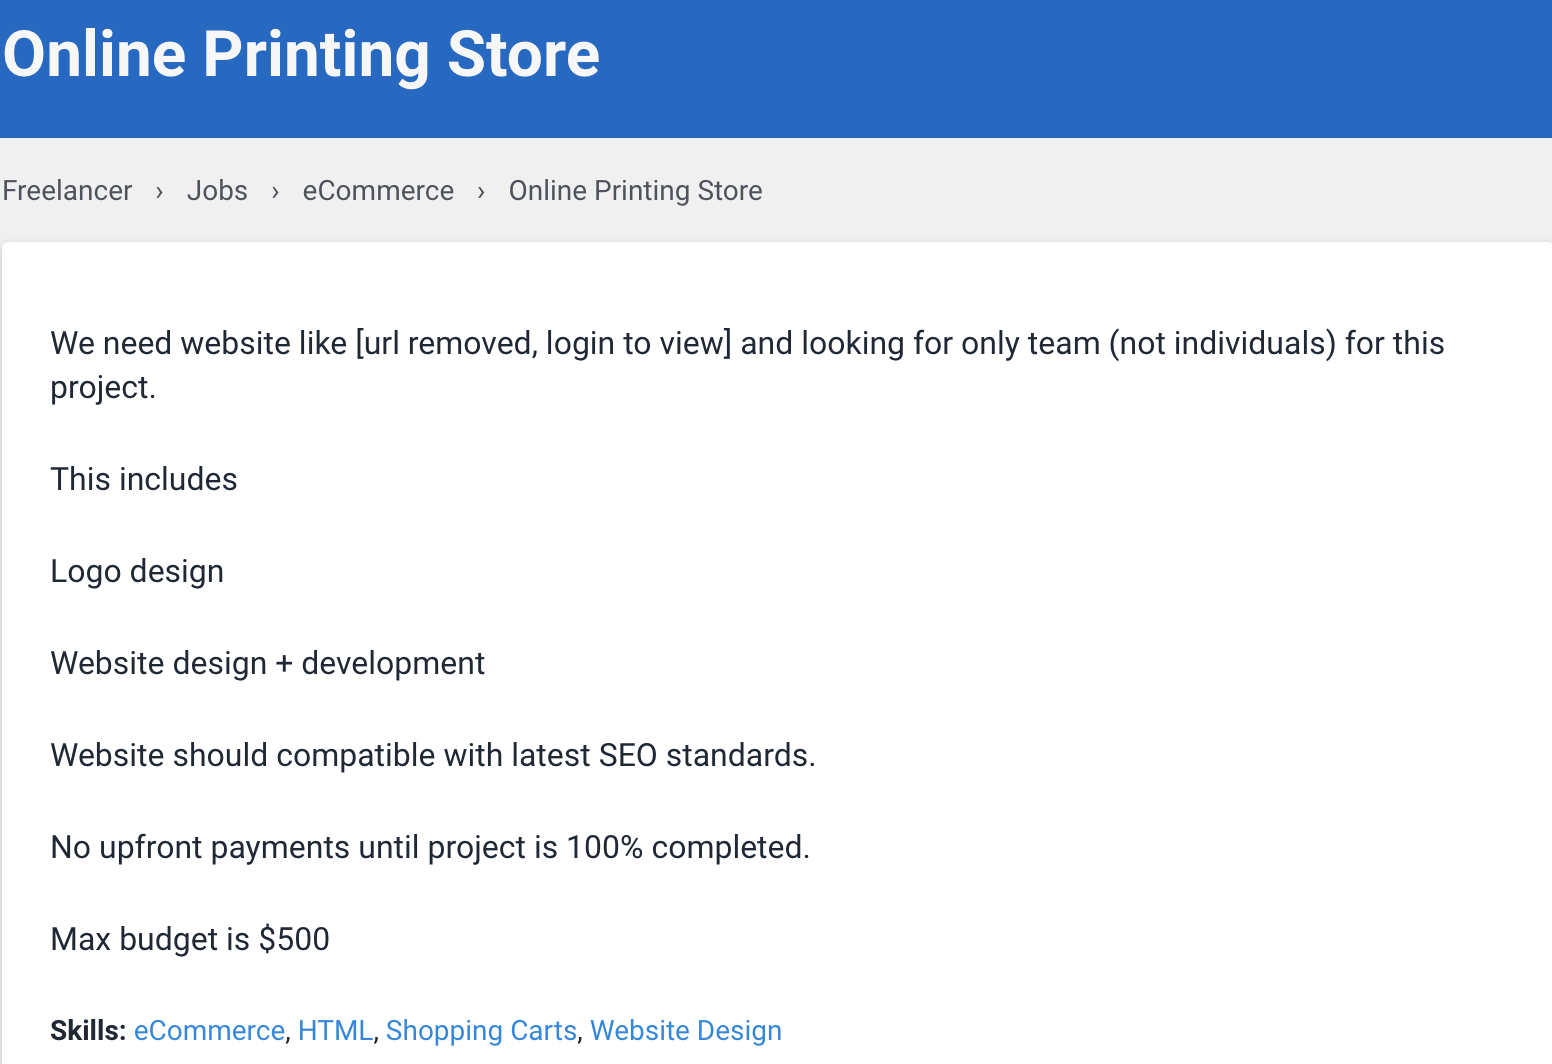
\includegraphics[width=\textwidth]{figures/FreelancerExample.png}
	\caption{An example project from the Freelancer Website}
	\label{fig:freelancer-example-project}
\end{figure}


As you can see in the figure \ref{fig:freelancer-example-project}, a typical freelancer project posting consists of a title, the description and the relevant skills. For simplicity, the thesis at hand only concentrates on the skills and doesn't take the project description into account. This would be topic of another paper/thesis, as it would require natural language processing and other techniques ~\parencite{bird2009natural}.


\begin{figure}[h]
	\centering
	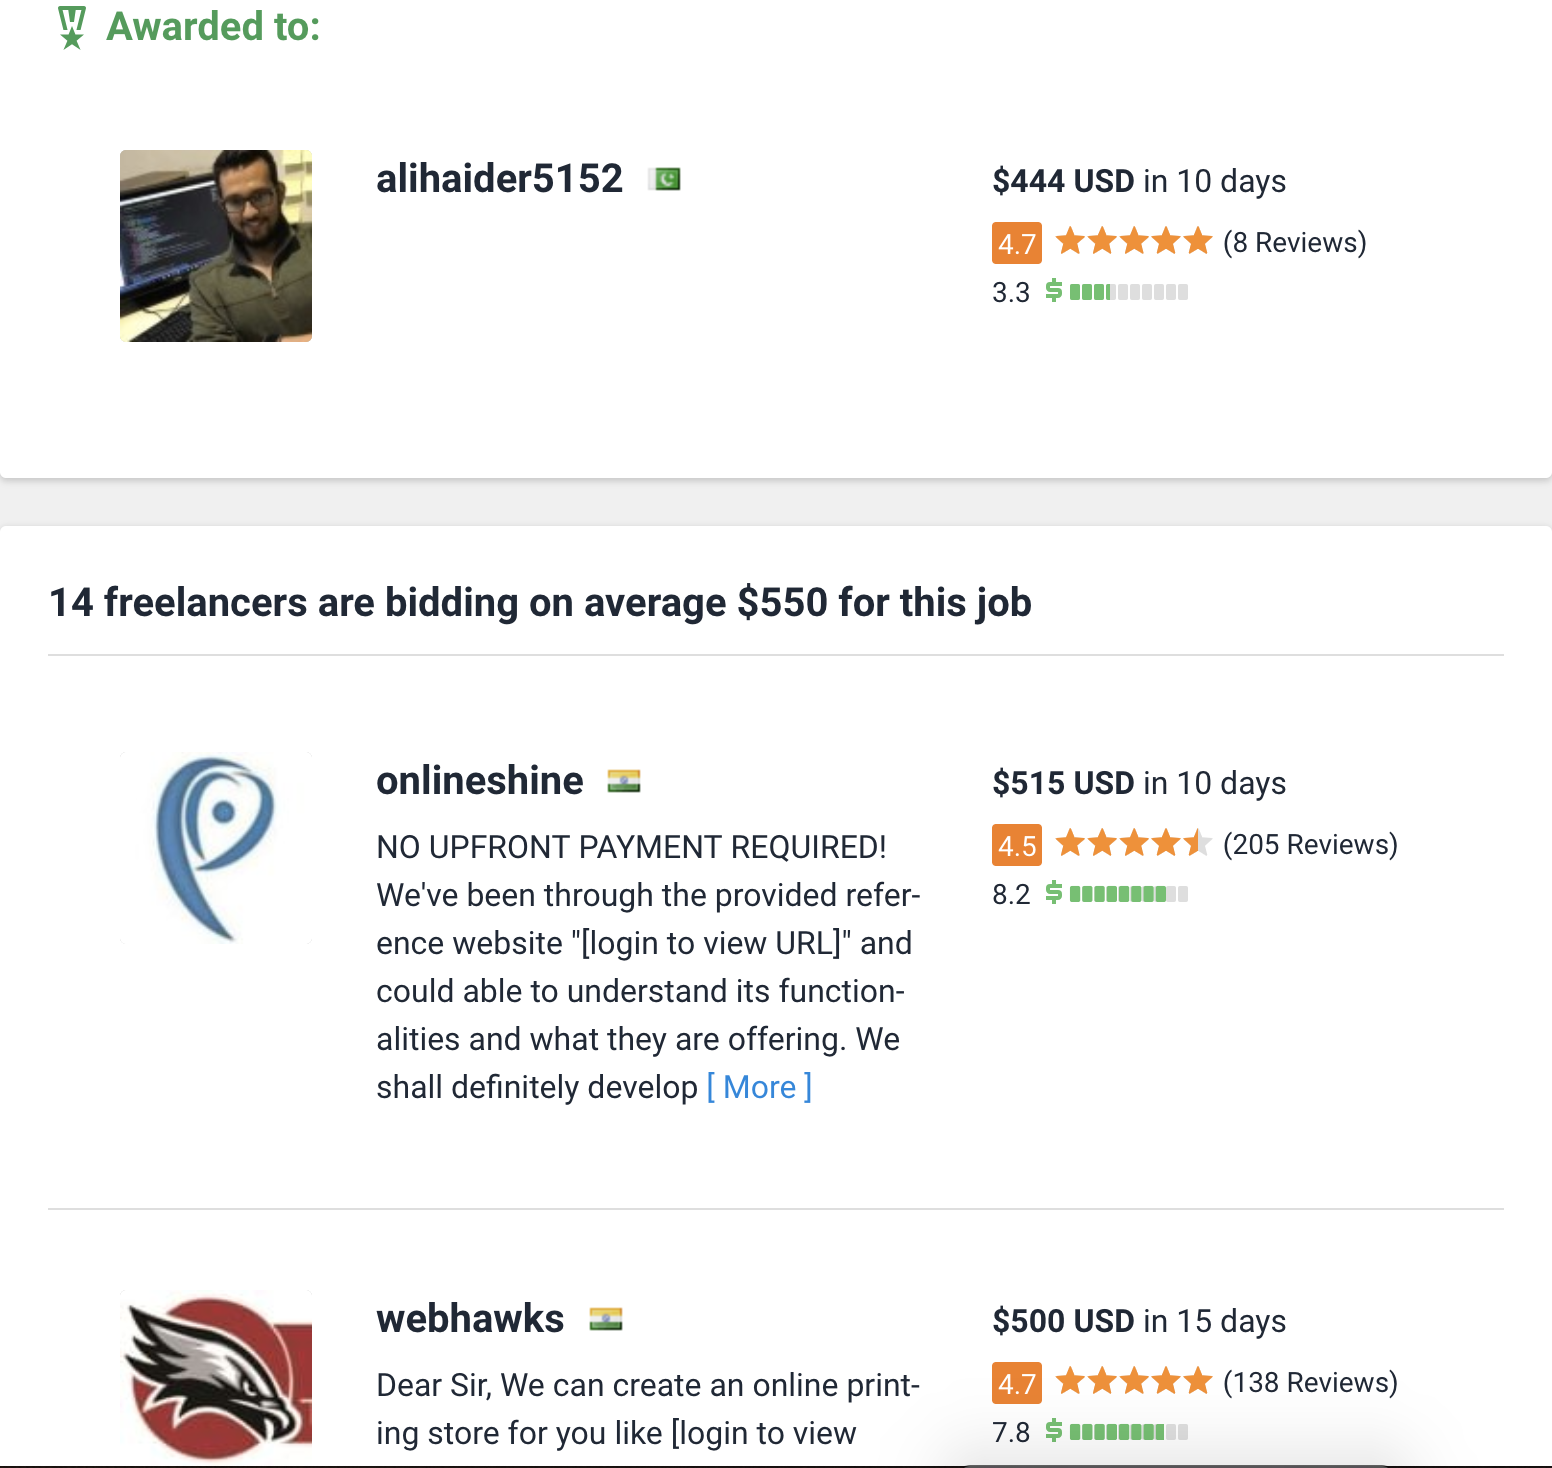
\includegraphics[width=0.75\textwidth]{figures/FreelancerTalentExample.png}
	\caption{The winner and other bidders to the same project}
	\label{fig:freelancer-example-talent}
\end{figure}


The figure \ref{fig:freelancer-example-talent} shows the bidders of the same project as above. The first one of the bidders has won the bidding race, which is decided by the creator of the project. The bidders include information such as a motivation text, the demanded monetary amount, their star rating until the time of bidding, amount of reviews they received and their total earnings until that date. In this thesis, we only consider the money they demand, their star rating and the number of reviews. For the sake of simplicity, we don't use the motivation text.


Each bidder lists their skills on their profile page and the employers may check their profiles before hiring talents. 

\begin{figure}[h]
	\centering
	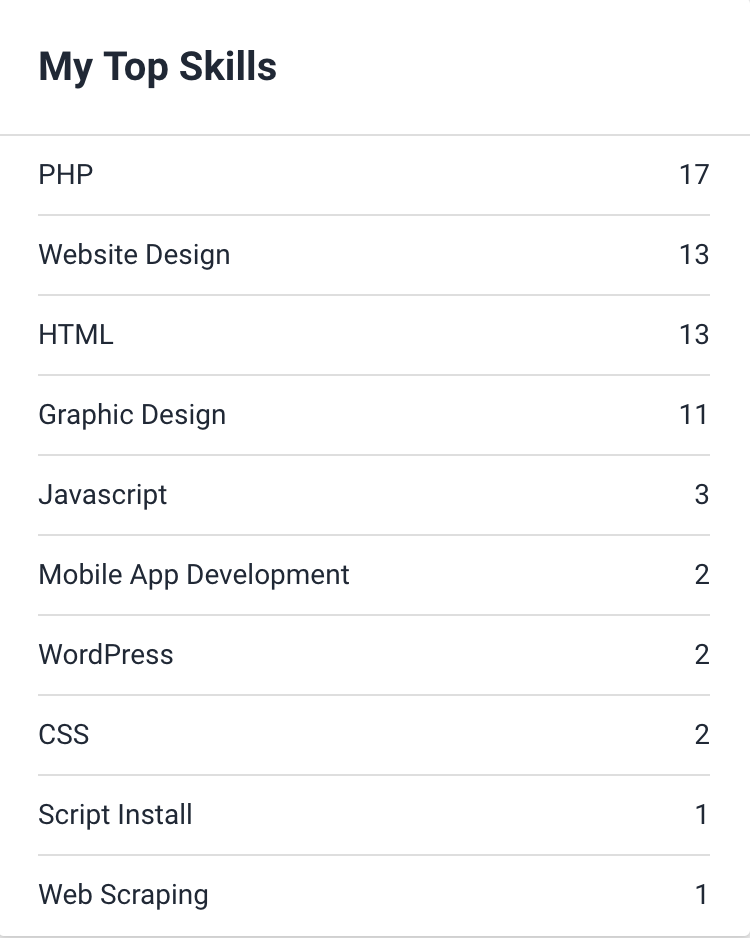
\includegraphics[width=0.5\textwidth]{figures/FreelancerTalentSkills.png}
	\caption{The list of tops skills by a talent on Freelancer web page}
	\label{fig:freelancer-talent-skills}
\end{figure}





\subsection{Company Dataset}\label{subsection:company-dataset}


\section{Unsupervised Individual Recommender}

\section{Supervised Individual Recommender}

\subsection{Using Sparse Input}

\subsection{Using Embeddings}

\subsection{Simpler Architecture for Company Dataset}

\section{Unsupervised Group Recommender}

\section{Supervised Group Recommender}

\subsection{Using Sparse Input}

\subsection{Using Embeddings}

\subsection{Using Clustering}

\subsection{Using Recurrent Neural Networks}

\section{Dashboard to show data and enter Feedback}

\section{Improvement of Recommendations via Feedback Learning}

\section{Conclusion}
